\documentclass[english,12pt,twoside,a4paper]{report}
    \usepackage[ngerman,english]{babel,varioref}		% Language specification
    \usepackage[utf8]{inputenc}
    \usepackage[T1]{fontenc}    % Required to output umlauts in a PDF
    \usepackage{pslatex}
    \usepackage{amsmath}
    \usepackage{multirow}
    \usepackage{ellipsis}
    \usepackage{textcomp}
    \usepackage{longtable}
    \usepackage{rotating}
    \usepackage[section]{placeins}

    \usepackage{caption}		% Customize caption aesthetics
    \usepackage{subcaption}

	\usepackage{xcolor}			% Highlighting
	\usepackage{tcolorbox}		% Fancy colored boxes
    \usepackage{soul}

    \usepackage[tracking=true]{microtype} % required to change character spacing

    \usepackage{listings}       % insert programming code
	\usepackage{graphicx}		% Required to insert images
	\usepackage[space]{grffile} % Insert images baring a filename which contains spaces
	\usepackage{float}			% Forcefully set the location of an object

	\usepackage[style=numeric,backend=biber]{biblatex}
	\usepackage[bookmarks]{hyperref}	% Clickable references

    %\usepackage[ddmmyyyy]{datetime}
	\usepackage{datetime}		% Flexible date specification
	\newcommand{\leadingzero}[1]{\ifnum#1<10 0\the#1\else\the#1\fi}
	\newcommand{\todayddmmyyyy}{\leadingzero{\day}.\leadingzero{\month}.\the\year}
	\newcommand{\mathcolorbox}[2]{\colorbox{#1}{$\displaystyle #2$}}

    \usepackage{geometry}
	\usepackage{scrextend}		% Arbitrary indentation

    \usepackage{color}

	\addbibresource{../literature.bib}

    \makeatletter
    \makeatother

    \pagestyle{headings}                 % Seitenstil
    \oddsidemargin0.8cm                  % linker Rand fuer ungerade Seiten bei \twoside
    \evensidemargin0.2cm                 % linker Rand fuer gerade Seiten (nur bei \twoside)
    \topmargin0.5cm                      % oberer Rand bis zur Oberseite Kopfzeile
    \textheight21cm                      % Texth"ohe auf einer Seite
    \textwidth15cm                       % Textbreite auf einer Seite
    \renewcommand{\topfraction}{0.75}    % Anteil der Gleitk"asten am Seitenanfang
    \renewcommand{\bottomfraction}{0.75} % Anteil der Gleitk"asten am Seitenende
    \parskip1ex  plus1ex minus0.5ex      % Abstand zwischen Abs"atzen
    \parindent0em                        % Einr"uckung der ersten Zeile eines Absatzes
    \newcommand{\clearemptydoublepage}{\newpage{\pagestyle{empty}\cleardoublepage}}

    \title{Optimization of Particle Identification}
    \author{\href{mailto:gordian.edenhofer@gmail.com}{Gordian Edenhofer}}
    \date{29. June 2018}

\begin{document}

\selectlanguage{english}

\pagenumbering{Roman}
%\maketitle
\thispagestyle{empty}
\begin{center}
	\selectlanguage{ngerman}

	\begin{LARGE}
		{
		\bf
		\hspace*{1cm} Optimierung der Teilchenidentifizierung \\ [0.3cm]
		}
	\end{LARGE}
	\vspace{0.5cm}
	%
	\begin{figure}[htbp]
		\begin{center}
			\hspace*{1cm}
			
\includegraphics[height=4cm]{{{../res/LMU logo}}}
		\end{center}
		%\label{fig-lmulogo}
	\end{figure}

	\vspace{1.0cm}
	\begin{large}
		\hspace*{1cm}Bachelorarbeit an der Fakultät für Physik \\
		\hspace*{1cm}der \\
		\hspace*{1cm}Ludwig-Maximilians-Universität~München \\ [2.5cm]

		\hspace*{1cm}vorgelegt von \\
		{
		\bf
		\hspace*{1cm}Gordian~Edenhofer \\
		}
		\hspace*{1cm}geboren in Frankfurt am Main am \datengerman\formatdate{13}{07}{1997} \\ [0.5cm]

		\hspace*{1cm}München, den \datengerman\formatdate{29}{06}{2018} \\ [0.5cm]

		\hspace*{1cm}Betreuer: \\
		{
		\bf
		\hspace*{1cm}Prof.~Dr.~Thomas~Kuhr
		}
	\end{large}
\end{center}

\clearpage
\thispagestyle{empty}
\mbox{ }
\setcounter{page}{0}
\clearpage
\thispagestyle{empty}
\begin{center}
	\begin{LARGE}
		{
			\bf
			\hspace*{1cm} Optimization of Particle Identification \\ [0.3cm]
		}
	\end{LARGE}
	\vspace{0.5cm}
	%
	\begin{figure}[htbp]
		\begin{center}
			\hspace*{1cm}
			
\includegraphics[height=4cm]{pics/lmu3.pdf}
		\end{center}
		%\label{fig-lmulogo}
	\end{figure}

	\vspace{1.0cm}
	\begin{large}
		\hspace*{1cm}Bachelor thesis at the faculty of physics \\
		\hspace*{1cm}of the \\
		\hspace*{1cm}Ludwig-Maximilians-Universität München \\ [2.5cm]
		\hspace*{1cm}handed in by \\
		{\bf
		\hspace*{1cm}Gordian Edenhofer \\ }
		\hspace*{1cm}born in Frankfurt am Main on the \formatdate{13}{07}{1997} \\ [0.5cm]
		%\hspace*{1cm}\today
		\hspace*{1cm}Munich, the \formatdate{28}{06}{2018}
	\end{large}
\end{center}

\clearpage
\thispagestyle{empty}
\mbox{ }
\setcounter{page}{0}
%\clearpage
%\chapter*{Abstract}

This study aims at evaluating further particle identification approaches.
At first the goodness of the detector variables is measured. Flaws are outlined and possible causes are evaluated. Afterwards further techniques are discussed which combine the detector variables in a new way.

A Bayesian approach to particle identification is discussed. It aims at producing probabilities of a track belonging to a particle species in dependance of the received signal. The process of obtaining the conditional probabilities is described in greater detail. In addition, some extensions to the Bayesian approach are presented and evaluated. Flaws and benefits are compared using a generic decay.

Lastly, a neural network is used to label particle tracks. For a simple network, different methods to adapt the weights and various input forms are evaluated. Hereby, tools from machine learning and statistics are discussed and their application is outlined. In the end the accuracy of the network on a generic decay is determined.

\clearpage

\tableofcontents

\cleardoublepage

\pagenumbering{arabic}

\chapter{Belle~\RN{2}}
\label{chap:belle2_experiment}

\section{Experiment}
\label{sec:experimental}

The Belle~\RN{2} experiment is performed at the SuperKEKB accelerator located in Tsukuba, Japan. It is mainly designed to study B mesons.
In the experiment, asymmetric electron- positron-beams are collided with a center of mass energy of $\sqrt{s} = 10.58 \mathrm{~GeV}$, exactly on the $\Upsilon (4S)$ resonance. The two beams, positrons at $4 \mathrm{~GeV}$ and electrons at $7 \mathrm{~GeV}$, are focussed to a narrow crossing section. The additional boost in one direction is used to measure the $B$ meson lifetimes.

In comparison to the predecessor experiment Belle, the integrated luminosity will be $50~{ab}^{-1}$ and hence $50$ times higher. The instantaneous luminosity will be $8 \cdot 10^{35} \mathrm{cm}^{-2} \mathrm{s}^{-1}$, which is a $40$-fold increase.

\section{Detector system}
\label{sec:detector_system}

\subsection{Overview}
\label{sec:detector_system_overview}

The Belle~\RN{2} detector system~\cite{Abe:2010gxa,Pulvermacher:SuperKEKBDetectorComponents,Pulvermacher:AnalysisSoftware} is a composition of multiple detectors, each measuring a subset of a particle's properties. Its design is depicted in~\autoref{fig:belle2_detector_design_white_paper}.
The inner three detectors -- \textbf{P}i\textbf{X}el \textbf{D}etector (PXD), \textbf{S}ilicon \textbf{V}ertex \textbf{D}etector (SVD) and \textbf{C}entral \textbf{D}rift \textbf{C}hamber (CDC) -- record the position of traversing charged particles. Hence they are also called tracking detectors. They are located in a homogeneous magnetic field of $1.5~\mathrm{T}$.
The innermost detector is the PXD. Together with the SVD which surrounds the PXD, it is used to reconstruct decay vertices and identify tracks belonging to particles with low-momenta.
The CDC measures the momentum and charge of particles via their curvature in the magnetic field.
Next, the \textbf{T}ime \textbf{O}f \textbf{P}ropagation counter (TOP) (`Barrel~PID') and the \textbf{A}erogel \textbf{R}ing-\textbf{I}maging \textbf{CH}erenkov (ARICH) counter (`Endcap~PID') are used to identify charged particles via their emission of Cherenkov radiation in the detector. However, there is no such installation for the backwards-facing endcap of the detector due to the asymmetric beams.
The \textbf{E}lectromagnetic \textbf{C}a\textbf{L}orimeter (ECL) identifies photons and electrons.
The outermost detector called $\boldsymbol{K}^0_{\boldsymbol{L}}$/$\boldsymbol{\mu}$ (KLM) is used to identify kaons and muons\footnotemark.
\footnotetext{If not specifically stated otherwise, the charge conjugate of a particle is implied.}

\begin{figure}[ht]
	\centering
	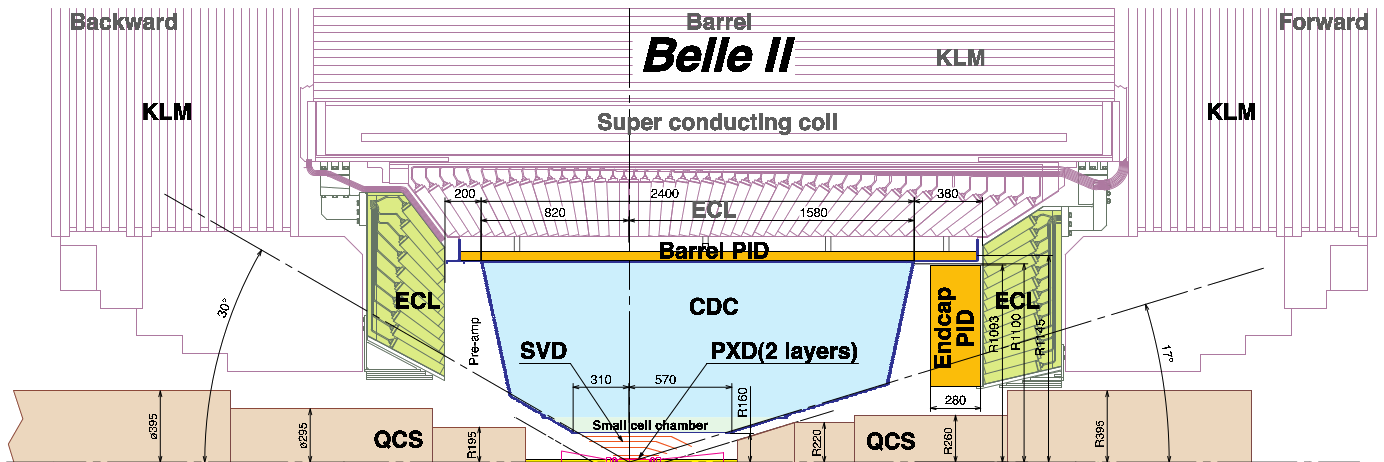
\includegraphics[width=\textwidth,height=0.6\textheight,keepaspectratio]{{{../res/Belle 2 detector design white paper (truncated)}}}
	\caption{Side view of the upper half of the Belle~\RN{2} detector. Adapted from~\cite{Abe:2010gxa}.}
	\label{fig:belle2_detector_design_white_paper}
\end{figure}

\subsection{Silicon detectors}
\label{sec:detector_system_silicon_detectors}

The PXD and SVD consist of tiny doped silicon chips which yield the location of electron-holes created by particles passing through it. The PXD detector uses small pixels while the SVD detector uses strips of detector material. Therefore, the PXD detector is able to further differentiate multiple simultaneous tracks while the SVD allows for a faster readout and is less prone to noise.

\subsection{Central drift chamber}
\label{sec:detector_system_tracking_detectors}

The CDC, which surrounds the PXD and SVD, consists of a collection of field wires and sense wires located in a volume filled with gas. The sense wires are used to measure the current produced by electromagnetic showers. The latter is caused by particles passing through the gas. The wires are close to being parallel to the beampipe but have a slight twist. This allows the detector to not only have an excellent estimation of the transverse distance to the beam pipe but also provides information about the longitudinal position.

\subsection{Barrel and endcap PID}
\label{sec:detector_system_barrel_and_endcap_pid}

The Cherenkov effect is used to measure the velocity of particles in the TOP and ARICH detector. Charged particles which travel faster than the speed of light in the medium -- Quartz in case of the TOP detector and aerogel for the ARICH detector -- produce light. The velocity can be calculated by measuring the time of propagation and the angle of the emitted light.

\subsection{Electromagnetic calorimeter}
\label{sec:detector_system_electromagnetic_calorimeter}

The main purpose of the ECL detector is to determine the energy of photons and electrons. Both particle species excite the medium and create electromagnetic showers. The light of the de-excitation can subsequently be measured.

\subsection{$\boldsymbol{K}^0_{\boldsymbol{L}}$/$\boldsymbol{\mu}$ detector}
\label{sec:detector_system_k0lmu}

Last but not least, the KLM detector identifies kaons and muons which have passed through the previous layers of the system. When traversing this detector, the particles pass through plates serving as electrodes separated by layers of gas in between them. Ionized particles are accelerated in this field and subsequently produce a spark picked up by the detector via measuring the drop in voltage.

\section{Interaction with matter}
\label{sec:interaction_with_matter}

\subsection{Charged particle interaction}
\label{sec:interaction_with_matter}

Particles with non-zero charge mainly interact with the medium electromagnetically. In general, an interaction occurs either by scattering in the electric field of the atom, polarization of the medium, ionization or excitation. Besides, hadrons may scattering at the atom itself. Particles and their anti-particles additionally have the ability to annihilate.

The polarization of the medium causes Cherenkov radiation to be emitted. At velocities below the speed of light in the medium ($v < c/n$), only boundaries of the particle's velocity may be determined. However, at $v > c/n$ the Cherenkov effect can be observed. The effect occurs due to the information about the charge of the traversing particle not reaching the medium in front of it soon enough. Hence, the medium behind the particle is already aligned with the electric field while the medium in front is not. The result is an electromagnetic wave. The angle between the normal vector of the wave and the track of the particle is given by
\begin{equation}
	\cos(\Theta_{c}) = \frac{1}{v/c \cdot n} = \frac{1}{\beta \cdot n}
	\mathrm{.}
\end{equation}
This is the effect which the TOP and ARICH detectors exploit.

Particles with low energy traveling through a medium interact predominantly with atomic electrons. The average energy loss of a particle is described by the Bethe-Bloch formula. It is given by $\left< \mathrm{d}E/\mathrm{d}x \right> \propto 1/{\beta^2}$ for velocities of up to about $90\%$ of the speed of light and is minimal at $\beta \gamma \approx 4$. It describes the momentum dependency of the average energy loss. However, the actual shape of $\mathrm{d}E/\mathrm{d}x$ is modelled by the Landau distribution. Note that the initial assumptions needed for this formula are not met for electrons. This is because both participants of the interaction belong to the same species and have identical masses.
A $\mathrm{d}E/\mathrm{d}x$-measurement is performed at the silicon detectors and the CDC.

The interaction with the electromagnetic field of the nucleus is the dominant cause for the energy loss of high-energy particles. Energy is radiated away via so called Bremsstrahlung. The leftover energy decreases exponentially with the distance traversed and is inversely proportional to the square root of the mass. Therefore it is mainly important for particles with a low mass, e.g., electrons. The radiation due to this effect is mainly measured by the ECL.

\subsection{Particle identification}
\label{sec:particle_identification}

At Belle~\RN{2} the detector system differentiates among six long living particle species $K, \pi, e, \mu, p \text{ and } \hbox{deuteron}$.

The $\mathrm{d}E/\mathrm{d}x$-measurement from the silicon detectors and the CDC are one of the most useful measurements. \autoref{fig:de_dx_for_SVD} showcases this for one of the tracking detectors for momenta below $1 \mathrm{~GeV/c}$. Distinct patterns may be observed for various particle species below this momentum threshold.
New tracks can now be assigned a likelihood of producing the measured detector signal given they belonging to a certain particle species. This is done by postulating a hypothesis for the loss of energy for each such species.

ARICH, TOP and CDC furthermore extend the identification and are able to differentiate among $K, \pi, p \text{ and } \hbox{deuteron}$ but also contribute to $e$ and $\mu$ identification. They provide likelihoods for each signal given a particle hypothesis.

Further out the ECL detector provides a good separation of electrons from other charged particles above $1 \mathrm{~GeV/c}$. It is able to do so via measuring $E/p$ of the shower. The detector response is provided by estimating the degree of agreement for different particle hypothesis with the signal. An exemplary $E/p$ curve is shown in \autoref{fig:e_p_for_ECL}. It demonstrates the observable difference for electrons compared to other particle species but also shows that no clear separation of pions and muons is possible.

The KLM detector provides a good separation between muons and non-muons and contributes to the discrimination in the form of different likelihoods as well.

\begin{figure}[ht]
	\centering
	\subcaptionbox{$\mathrm{d}E/\mathrm{d}x$\label{fig:de_dx_for_SVD}}{
		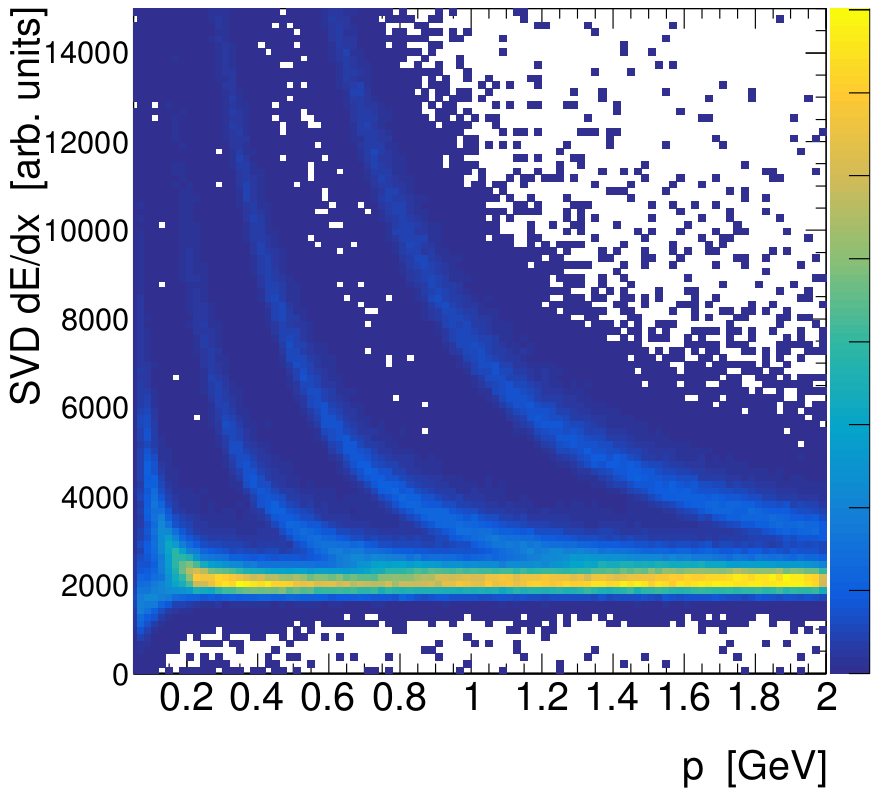
\includegraphics[width=0.43\textwidth,height=\textheight,keepaspectratio]{{{../res/dE dx for SVD detector by particles}}}
	}
	\hspace{2em}
	\subcaptionbox{$E/p$\label{fig:e_p_for_ECL}}{
		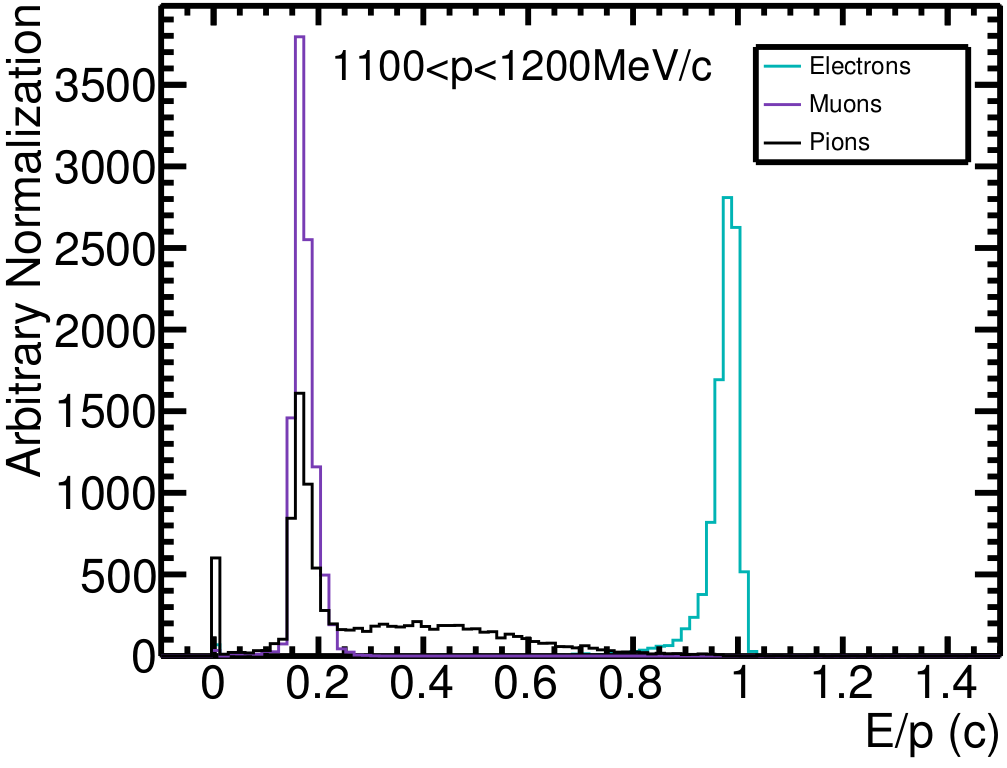
\includegraphics[width=0.43\textwidth,height=\textheight,keepaspectratio]{{{../res/E p for ECL detector by particles}}}
	}
	\caption[Separation of different particle species for various simulated signals. Taken from~\cite{Belle2Collaboration:B2TiP}.]{
		Separation of different particle species for various simulated signals. Taken from~\cite{Belle2Collaboration:B2TiP}.

		\textbf{Figure~\subref{fig:de_dx_for_SVD}} shows the $\mathrm{d}E/\mathrm{d}x$ means as a function of momentum in the SVD with the color encoding the number of hits. In order to reduce outliers the lowest $5\%$ and highest $25\%$ of the measurements of each track are not used in the estimation.

		\textbf{Figure~\subref{fig:e_p_for_ECL}} shows the $E/p$ distribution for different particle species.
	}
\end{figure}

\chapter{Statistics for particle analysis}
\label{chap:statistics}

\section{Classification functions}
\label{sec:classification_functions}

A main part of identifying particles is to examine statistical measures. The main concepts used throughout the thesis heavily relies on such values to compare the goodness of a identification method. However their use is not limited to physics, let alone particle physics, but spans over all field containing some form of (binary) classification problems.
In the following explanatory paragraphs it is assumed that one wants to identify kaons in a set of data containing a multitude of alternative particles.

The most important classification functions are:
\begin{itemize}
	\item \textbf{T}rue \textbf{P}ositive \textbf{R}ate (\textbf{TPR}): \textit{Proportion of accepted elements which are correct relative to all positives}

	\nobreak
	Hence the ratio of identified kaons which actually were kaons in proportion to the number of kaons in the data.

	\item \textbf{T}rue \textbf{N}egative \textbf{R}ate or Specificity (\textbf{TNR}): \textit{Proportion of rejected elements which are incorrect relative to all negatives}

	\nobreak
	In our example this would translate to the ratio of non-kaon particles being identified as non-kaons in proportion to the number of all non-kaon particles.

	\item \textbf{F}alse \textbf{P}ositive \textbf{R}ate (\textbf{FPR}): \textit{Proportion of accepted elements which are incorrect relative to all negatives}

	\nobreak
	This would translate to the fraction of non-kaon particles identified as kaons over the number of all non-kaons.

	\item \textbf{F}alse \textbf{N}egative \textbf{R}ate (\textbf{FNR}): \textit{Proportion of rejected elements which are correct relative to all positives}

	\nobreak
	Using our kaon sample once more; this would represent the fraction of kaons classified as being non-kaons over the number of all non-kaons.

	\item \textbf{P}ositive \textbf{P}redicted \textbf{V}alue (\textbf{PPV}): \textit{Proportion of accepted elements which are correct relative to all accepted}

	\nobreak
	Using our kaon sample one last time; this would represent the fraction of kaons classified as being as kaons over the number of all tracks classified as kaons but not necessarily being one.

\end{itemize}

In abstract terms; the two prefixes used above may be summarized as seen in \autoref{tab:classification_guidelines}. Bear in mind that `negative' and `positive' if used separately denote the presence of the desired feature and therefore does not fit the definition given in the table in this case.

\begin{table}[ht]
	\centering
	\begin{tabular}{l|ll}
		Veracity & True = correct & False = incorrect \\
		Identification & Positive = accepted & Negative = rejected
	\end{tabular}
	\caption{Guidelines for understanding the meaning of a classification function.}
	\label{tab:classification_guidelines}
\end{table}

\section{Receiver operating characteristic}
\label{sec:roc}

The \textbf{R}eceiver \textbf{O}perating \textbf{C}haracteristic (\textbf{ROC}) curve is the TPR plotted over the FPR. As such the values on the $x$ and $y$ axis go from $0$ to $1$. Each point on the curve represent an applied selection criterion on the data.

On a set of data with two equally likely yields a straight diagonal line connecting the point $(0, 0)$ with $(1, 1)$ would represent plain guessing. A curve below that would be worse and anything above, is some degree of good. An optimal curve would achieve a high TPR value at a very low FPR.
Multiple methods can therefore be compared by assessing how steep each methods TPR is rising relative to the FPR. The \autoref{fig:sample_roc_curve} visually underlines the above described relations.

\begin{figure}[ht]
	\centering
	\includegraphics[width=\textwidth,height=0.4\textheight,keepaspectratio]{{{../res/Sample Receiver Operating Characteristic (ROC) curve}}}
	\caption{Sample ROC curve for a binary classification problem with each outcome being equally likely.}
	\label{fig:sample_roc_curve}
\end{figure}

\section{Identification efficiencies}
\label{sec:efficiency}

In particle physics the identification efficiency is defined as the proportion of correctly classified particles relative to all the available particles belonging to that class. Hence it directly represents the PPV. Both terms will be used as synonyms throughout the thesis.

For an exclusive particle classification the $\epsilon_{PID}$-matrix is the confusion matrix normed by row. Each cell in a row represents the probability of a particle of that row's class being identified as the particle of that column's class. On the diagonal of that matrix it contains the identification efficiencies for a particle species.
The definition generalizes to non normed matrices, e.g. resulting from non-exclusive. Although reading the matrix is less intuitive as a particle might belong to multiple classes and makes comparing them very ambitious.

The values of the matrix are given by the fraction of particles $i$ classified as $j$ over the true abundance of particle $i$. As formula its values are

\begin{equation}
	\epsilon_{i j} = \frac{N_{i \text{ classified as } j}}{A_{i \text{ true}}}.
\end{equation}

For our six particle species with ID the matrix has the following shape:

\begin{equation}
	\begin{pmatrix}
		\epsilon_{K K} & \epsilon_{K \pi} & \epsilon_{K e} & \epsilon_{K \mu} & \epsilon_{K p} & \epsilon_{K d} \\
		\epsilon_{\pi K} & \epsilon_{\pi \pi} & \epsilon_{\pi e} & \epsilon_{\pi \mu} & \epsilon_{\pi p} & \epsilon_{\pi d} \\
		\epsilon_{e K} & \epsilon_{e \pi} & \epsilon_{e e} & \epsilon_{e \mu} & \epsilon_{e p} & \epsilon_{e d} \\
		\epsilon_{\mu K} & \epsilon_{\mu \pi} & \epsilon_{K e} & \epsilon_{K \mu} & \epsilon_{K p} & \epsilon_{\mu d} \\
		\epsilon_{p K} & \epsilon_{p \pi} & \epsilon_{p e} & \epsilon_{p \mu} & \epsilon_{p p} & \epsilon_{p d} \\
		\epsilon_{d K} & \epsilon_{d \pi} & \epsilon_{K e} & \epsilon_{K \mu} & \epsilon_{K p} & \epsilon_{d d} \\
	\end{pmatrix}.
\end{equation}

\section{Likelihood}
\label{sec:likelihood}

\subsection{Likelihood ratio}
\label{subsec:likelihood_ratios}

The ratio of likelihoods is commonly used for comparisons of the goodness of two models. Consider two alternative models, one parameterised by the hypothesis $H_0$, the other by $H_1$. Each yield a likelihood of event $\pmb{x}$ occurring given their hypothesis is true. Their ratio
\begin{equation*}
	\frac{\mathcal{L}(\pmb{x}|H_0)}{\mathcal{L}(\pmb{x}|H_1)}
\end{equation*} denotes how many times more likely the event $\pmb{x}$ is under hypothesis $H_0$ relative to $H_1$.

However the event $\pmb{x}$ must not necessarily take the form a simple one dimensional value. It may very well be a composition of e.g. in our case multiple detectors responses. Nevertheless if one assumes all constituents $x_i$ of $\pmb{x}$ are independent of each other, one may simple construct $\mathcal{L}(\pmb{x}|H_0)$ by multiplying the separate likelihoods of each $x_i$ given that $H_0$ is true:
\begin{equation*}
	\mathcal{L}(\pmb{x}|H_0) = \prod \limits_{i} \ell_i(x_i|H_0).
\end{equation*}
In out case $\mathcal{L}(\pmb{x}|H_0)$ might be seen as the likelihood of measuring a signal given a particle hypothesis is true. It value would be constructed by multiplying the likelihoods of $\ell(x_i|H_0)$ for each detector $i$.

\subsection{Neyman-Pearson}
\label{subsec:likelihood_ratios_neyman_pearson}

When separating two models which have no unknown parameters the Neyman-Pearson lemma states that a test on the likelihood ratio has the highest probability of correctly rejecting the original hypothesis if the alternative hypothesis is indeed true. In other words it states that a test on the likelihood ratio providing the highest purity at a given efficiency.

\section{Neural network}
\label{sec:neural_network}

A neural network or more precisely an artificial neural network is an algorithm inspired by the central nerve system of biological beings. However instead of electrical signals being passed on from neuron to neuron with complex biological process involved in summing up incoming systems, an artificial neural network passes on numbers with functions representing neurons.

Despite this simplistic design a neural network can get complicated fast. The most simplest approach would be to just stacking multiple layers of neurons (\textit{nodes}) on top of each other and connecting the outputs of the previous layer with those new nodes (feed-forward neural network). However a network can in theory be designed arbitrarily deep and provide a multitude of additional feedback loops (recurrent neural network) and further binning restrictions of node-inputs (convolutional neural network).

\begin{figure}[ht]
	\centering
	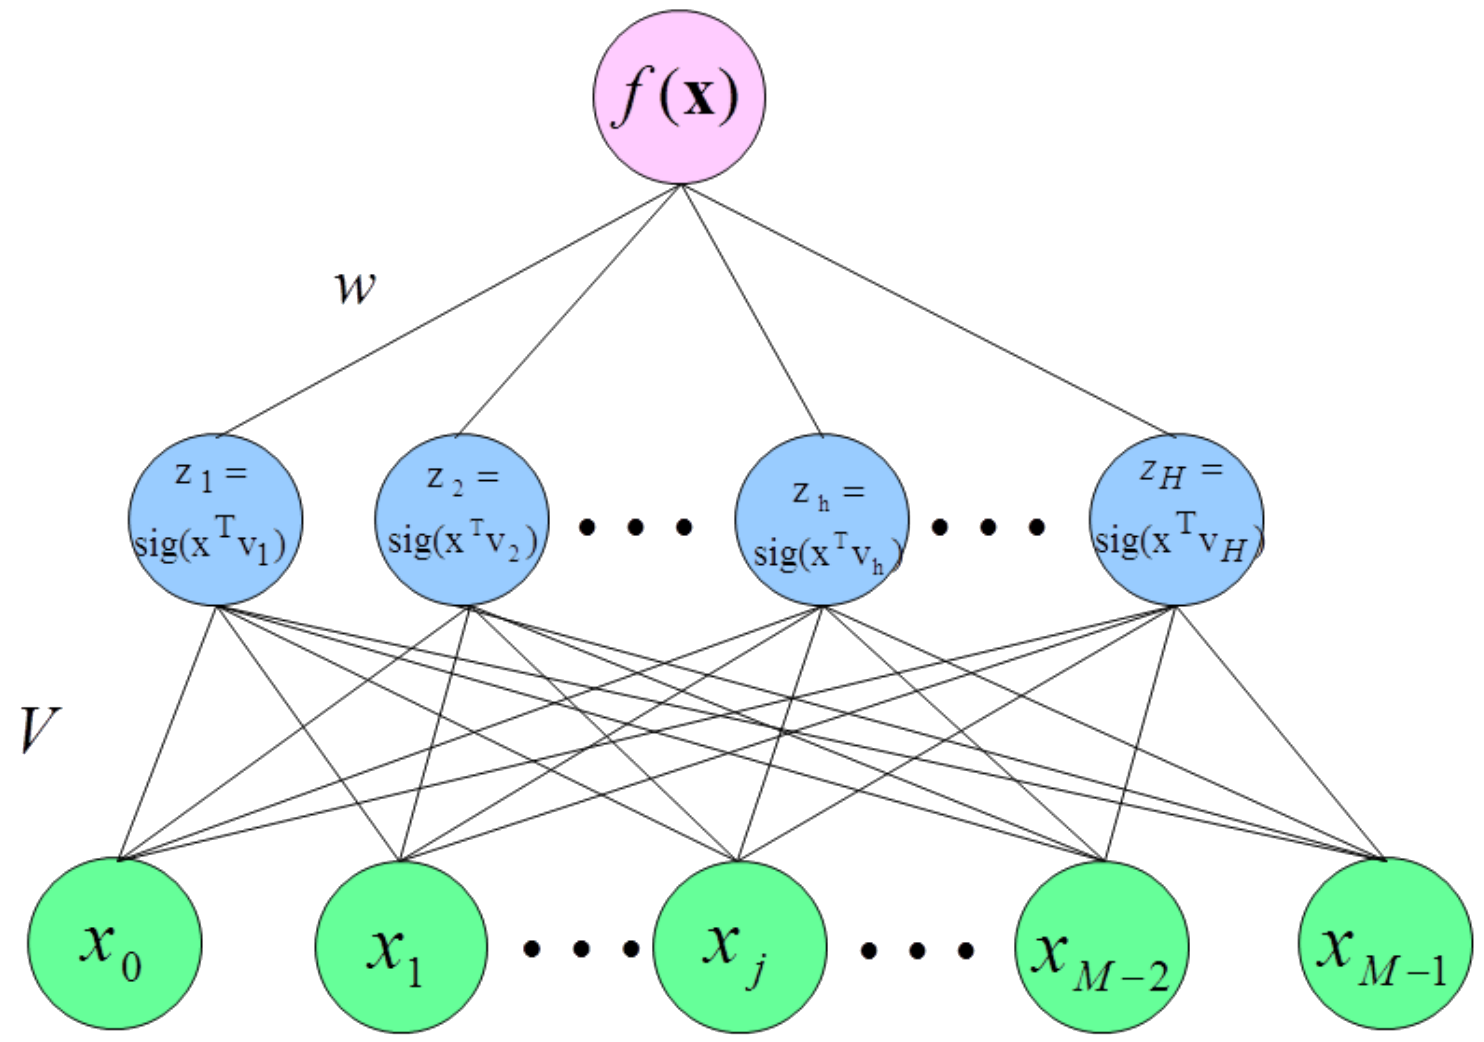
\includegraphics[width=\textwidth,height=0.4\textheight,keepaspectratio]{{{../res/Design of an artificial neural network}}}
	\caption{Design of an artificial neural network with one layer, $\pmb{x}$ as input, $z_i$ as activation function, $V$ und $w$ as weights and $f(\pmb{x})$ as prediction. Taken from~\cite{MachineLearning:NeuralNetworks}.}
	\label{fig:sample_neural_network_design}
\end{figure}

A rather simple feed-forward network is depicted in \autoref{fig:sample_neural_network_design}. Each line between two bubbles represents a connection, meaning the output of the bubble at the bottom is passed to the bubble at the top. The function used in calculating the various values for $z_i$ is called sigmoid (see~\cite{MachineLearning:NeuralNetworks}) and has an S-like shape. In terms of biology it can be though of as a boundary which has to be overcome prior to a signal being passed on. The references in the following paragraph are in regards to this figure.

Layers not representing the input or output are called hidden layers ({\color{blue}blue bubbles}). However the dimensions of an input ({\color{green}green bubbles}) are also referred to as features. The function of a node is called \textit{activation function} ($z_i$). The term \textit{learning} in the context of neural network refers to the process of adapting parameters or \textit{weights} ($V$ and $w$) of a nodes via a gradient which optimizes the desired function. The desired function is usually referred to as \textit{loss} and e.g. describes how many false classifications have been made. It is the job of the \textit{optimizer} to adapt the weights in a way which minimizes the function, a task usually done via propagating the error back through the network in a schema called \textit{back propagation}. The term \textit{training} refers to the process of applying the network to a set of data and adjusting the weights as necessary for each iteration. How many individual data points one of those iterations contains is described by the \textit{batch size}.

\chapter{Bayesian approach}
\label{chap:bayesian_approach}

\section{Simple Bayesian approach}
\label{sec:simple_bayes}

The goal of a Bayesian approach is to weight the particles' probability by their abundance in the sample. This process increases the likelihood of a particle being identified as belonging to a group with a higher abundance and decreases the likelihood of being identified as belonging to a group with a lower abundance. The approach depends on the detector yielding decay-agnostic results. Hence the detector shall be assumed to always output the likelihood of measuring the received signal given a specific particle hypothesis regardless of prior probabilities. Furthermore the approach assumes a bias towards one or a few particles in the sample since otherwise the a priori probabilities would be flat and therefore boil down to the same result.
Thankfully both of those hypothesis are given in the real world: The detector can be assumed to behaves independently of the relative particle abundance and the measured data usually shows a clear predominance of one or a few particle species.
This is not surprising in itself as the branching fractions are not equally distributed. Dictated by the laws of physics one particle species might be produced more frequently.

\begin{figure}[ht]
    \centering
    \includegraphics[width=\textwidth,height=0.4\textheight,keepaspectratio]{{{../res/charged 01/General Purpose Statistics: True Particle Abundances in the K+-Data}}}
    \caption{True particle abundance in the charged MC9 simulated data. \textit{NaN} stands for an invalid translation\protect\footnotemark from the particles' PDG code to an actual particle.}
    \label{fig:true_particle_abundance}
\end{figure}
\footnotetext{The error occurs due to the PDG code in the ROOT file being saved as \lstinline|float32| but some particle's code exceed the memory limit of $32$-bits. Notably, this effects the deuteron as well as its anti-particles.}

The absolute particle abundance of a sample taken from the Monte Carlo simulation of the charged decay of the $B$-mesons can be seen in \autoref{fig:true_particle_abundance}. In this example the bias towards pions and kaons can be clearly observed.

\begin{figure}[ht]
    \centering
    \includegraphics[width=\textwidth,height=0.4\textheight,keepaspectratio]{{{../res/charged 01/Diff Statistics: K Identification via PID, via flat Bayes}}}
    \caption{Comparisons of PPV and TPR for the Bayesian and standard PID approach for identifying kaons. The upper graph shows both rates of each approach separately using different colors, while the lower visualizes the ratio between the PPV's respectively the TPR's.}
    \label{fig:diff_stats_K_identification_via_pid_via_flat_bayes}
\end{figure}

\autoref{fig:diff_stats_K_identification_via_pid_via_flat_bayes} shows a comparison of the standard PID approach to the discussed Bayesian one. Using the Bayesian approach for identifying particles yields a very high positive predicted values even for low false positive rates as the introduced bias in the particle classification can utilize the unbalanced abundances. Furthermore the true positive rate of the Bayesian approach has a much steeper increase in comparison to the PID's one. However it levels of quicker, indicating that it fails to identify a few particles even at a high false positive rate.
The described effect can be seen for every stable particle with an ID and is not limited to the kaon. However it serves as a good example as it provides sufficient statistics for a throughout analysis.

\begin{figure}[ht]
    \centering
    \includegraphics[width=\textwidth,height=0.4\textheight,keepaspectratio]{{{../res/charged 01/Diff Heatmap: Heatmap of epsilonPID Matrix for an exclusive Cut via PID, via simple Bayes}}}
    \caption{Comparisons of the row-wised normed confusion matrix for the Bayesian and standard PID approach.}
    \label{fig:diff_heatmap_via_pid_via_flat_bayes}
\end{figure}

The improvements in the identification efficiencies are less obvious for an exclusive cut on the identifying variables. However in general the Bayesian approach is less prone to confusing particle with one another as seen in \autoref{fig:diff_heatmap_via_pid_via_flat_bayes}.

\section{Univariate Bayesian approach}
\label{sec:univariate_bayes}

The univariate Bayesian approach adds an dependency to one detector variable to the previous simple Bayesian approach. Hence instead of having a probability which depends on only on the particle abundance and the signal, the univariate approach additionally varies the probability depending on e.g. the transverse momentum. The most sensible variables are among others are said transverse momentum $p_t$ and the angle between the track of the particle and the beampipe $\Theta$.


\begin{appendix}
    %==================================================================
%\chapter{Anhang}
%==================================================================

%\label{sec-append}

%something
    \printbibliography
\end{appendix}
\pagestyle{empty}
\cleardoublepage
\section*{Disclaimer}

\thispagestyle{empty}
\vspace*{0.8\textheight}
\noindent
I confirm that this \MakeLowercase{thesis} is my own work and I have documented all sources and material used.

\vspace{15mm}
\noindent
%\getSubmissionLocation{}, \getSubmissionDate{} \hspace{50mm} \getAuthor{}

\cleardoublepage{}

\cleardoublepage
\thispagestyle{empty}
\chapter*{Acknowledgments}

This thesis would not have been possible without the continues support of numerous people. First of all, I would like thank my supervisor Prof.~Dr.~Thomas~Kuhr for the chance to work in his research group as a Bachelor's student. By providing helpful and constructive feedback at every opportunity, he gave me inspiring insights into various topics of experimental particle physics. Of cource, I would also like to thank James~Kahn and Dr.~Martin~Ritter for providing profound answers to all of my questions.
Specifically, I would like to thank Dr.~Michael~Bender, Dr.~Martin~Ritter and Jakob~Roth as well for proofreading my thesis and giving valuable feedback.

Furthermore, thank you to all the students at the working group of Prof.~Dr.~Kuhr for their welcoming attitude and for making my stay an enjoyable time. Thank you, Christoph Ames, Anna Bertolini, Nan-Hee Kang, Yasin Silyanoglu, Daniel Moritz and Jakob Roth.

Last but not least, I would like to thank my family which has always supported me in countless ways.

Thank you all!


\end{document}


